\documentclass[a4paper, 12pt, one column]{article}

\usepackage[english]{babel}
\usepackage[utf8x]{inputenc}
\usepackage[T1]{fontenc}

\usepackage[top=1.3cm, bottom=2.0cm, outer=2.5cm, inner=2.5cm, heightrounded,
marginparwidth=1.5cm, marginparsep=0.4cm, margin=2.5cm]{geometry}

\usepackage{graphicx} 
\usepackage[colorlinks=False]{hyperref} 
\usepackage[fleqn]{amsmath}  
\usepackage{amsfonts} 
\usepackage{amssymb} 
\usepackage{enumitem}
\usepackage{braket}
\usepackage{mathtools}

\newcommand\given[1][]{\:#1\vert\:}

\usepackage[authoryear]{natbib}
\bibliographystyle{abbrvnat}
\setcitestyle{authoryear,open={(},close={)}}
\title{CS 440 : Intro to Artificial Intelligence \\
\large Fast Trajectory Replanning}
\author{Devvrat Patel and Shubham Mittal}
\date{October 14, 2019} 

\setlength{\parindent}{4em}
\setlength{\parskip}{0.5em}
\begin{document}
\maketitle

\newpage

\begin{abstract}
For this project we created a program that will the best way possible for a robot to reach it's goal from a random starting point. We used Python to write the code for this project. To run this program you'll have to create the mazes using the ... (Add More stuff here) 
\end{abstract}


\section*{Part 0}

	To create a maze 101x101 , we start first with generating a numpy array with all zeros 
	Then start with generating paths reachable from neighbor points using 
	the random first depth search algorithm, start with a random coordinate 
	preparing a visited set , that will add each processed and finished 
	coordinate in that set till all cells of the map are visited.
	inside a loop , each time a random coordinate is selected from the neighbors of the last processed cell , and a uniform random number is generated between 0 and 1
	Once that uniform random number < 0.3 then the cell is blocked 
	and with 70% it is not blocked then add the visited coordinate to the stack 
	if reach dead end point (no unvisited cell in the neighbors) then pop from the stack till reach a cell that have other unvisited neighbors , then choose a random coordinate again from neighbors.
	If at sometime the stack is get empty then start the whole algorithm from a new point 
	Sample of a generated maze is shown in the following image :
	
	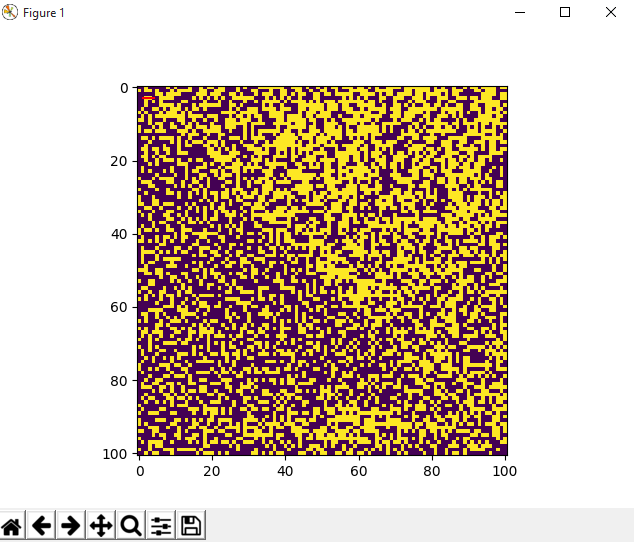
\includegraphics{SampleMaze.png}


\section*{Part 1}
  \begin{enumerate}[label=\alph*]
    \item 
      \begin{flushleft}
        The goal of this program is to find the shortest track for the agent to travel to the destination at Cell E5. In this example the agent's starting cell is Cell E3. At this point the agent has four option. The agent will not go South as Cell E3 is at the bottom edge. It will not go to West or North as they are both blocked. So the only optimal choice left for the agent is to move East which is exactly what it does. 
        \end{flushleft}
    \item 
    \begin{flushleft}
   There are multiple ways we can prove this. The simplest one would be that the number of grids is finite so the agent is bound to reach the goal. The worst case scenario here would be that the agent has to traverse the entire map. Also, A* has a close list, so the agent will never expand the cells that are previously expanded. This solves the issue of an infinite looping. To solve the problem of the goal blocked, the program will stop executing once every cell has been expanded. Therefore, if the goal is blocked by other cells then the program will just stop executing. 
    \end{flushleft}
  \end{enumerate}
  

  
\section*{Part 2}
        After implementing both versions of Repeated Forward A* we realized that the smaller g-value was worse compared to the larger g-values in terms of the number of nodes and run time.
        This happens because the algorithm with smaller g-value will expand a lot more cells near the start in the beginning. This caused the run time for the larger g-value to be noticeably faster than the one with smaller g-value.
   
        \par The algorithm with smaller g-value will be 15 slower than the one with larger g-value

\section*{Part 3}
        After all the comparisons between the two we realized that both the algorithms are fairly similar run time and expanded nodes. Even though the distance was the same for both the algorithm we noticed that Repeated Backward A* was quicker and had lesser expanded nodes compared to Repeated Forward A*. We found that the run time was faster and had 10 Percent lesser expanded cells. 
  
  
\section*{Part 4}
  \begin{enumerate}[label=\alph*]
    \item 
      \begin{flushleft}
      Manhattan distance is the distance between the two points on a grid and is strictly based on horizontal and/or vertical path. In the grid world, the agent only has four directions to move, that is up, down, left and right. Manhattan distance is the fastest path possible for the agent to reach it's goal. Since, the agent can not move diagonally, we can confirm that the shortest path will always be found and therefore Manhattan distance is consistent. If the agent could diagonally though, then heuristic would overestimate the distance. 

      \end{flushleft}
    \item 
    \begin{flushleft}
    A heuristic h(n) is consistent if, for every node n and every successor n’ of n generated by any action a, the estimated cost of reaching the goal from n is no greater than the step cost of getting to n’ plus the estimated cost of reaching the goal from n’. Therefore, if there is an action cost increase, then let's say c would be the cost before the increase and c' be the cost after it. Now to prove our point we will use the identity that 
    h(n) <= c(n,a,n') + h(n')
    Therefore, the hnew(n) <= hnew(n') + c(n,a,n') <= c'(n,a,n')
    Here, we can see that heuristic is consistent. 
 
    \end{flushleft}
  \end{enumerate}
  
\newpage  
\section*{Part 5}
        After implementing both the algorithms we noticed that the run times are fairly similar. However, the adaptive A* is still faster than Repeated Forward A* by (INSERT NUMBER). The number of nodes were also almost the same for the algorithms. Adaptive A* was almost 4 Percent better than the Repeated Forward A*. Through these numbers we can say that Adaptive A* is better than Repeated Forward A*. 
        


\section*{Part 6}
    For this program we used two different 2D arrays to store the f and g values of all the cells. Each array uses about 1 MByte of memory making it a total of 2 MByte for 1001x1001. We only stored the information about the cells which are visited in the arrays thus saving memory.  \par The largest grid using 4 MB will be roughly of size 1414x1414. For creating a gird of the size of 1001x1001 would take almost 2 MB.
  
\newpage
\bibliographystyle{plainnat} % or try abbrvnat or unsrtnat
\bibliography{}
  Binary Heaps,
  url = {https://runestone.academy/runestone/books/published/pythonds/Trees/BinaryHeapImplementation.html}
  \\
  \\
  Basic A* Information,
  url = {https://www.geeksforgeeks.org/a-search-algorithm/}
  \\
  \\
  Real-Time Adaptive A*,
  url = {http://idm-lab.org/bib/abstracts/papers/aamas08b.pdf}
  
  
  


      
\end{document}